Vor dem Lebensende des Adobe Flash-Players im Dezember 2020 wurde dieser häufig zur Entwicklung von browserbasierten Mehrspielerspielen verwendet. Diese Spiele wurden auf verschiedenen Plattformen wie zum Beispiel \textit{Newgrounds.com} oder \textit{Itch.io} angeboten. Der Flash-Player verfügte über Peer-To-Peer Fähigkeiten via Adobes \acf{RTMP}, beziehungsweise dem \acf{RTMFP}. \acs{RTMP} basiert auf \acs{TCP}, \acs{RTMFP} auf \acs{UDP}-Verbindungen. Für die Signalisierungsmechanismen nutzte der Flash-Player \textit{Adobe Cirrus} (non-kommerziell) oder den \textit{LiveCycle Collaboration Service} (komerziell) \cite{adobep2p}. Damit bot der Flash-Player als Plattform für Mehrspielerbrettspiele eine kostengünstige Alternative zur Nutzung von Client-Server Netzwerkarchitekturen. Mit dem Wegfall des Flash-Players ist WebRTC nun die einzige Technologie, welche ohne zusätzliche Software oder Plugins zum direkten Vernetzen von Browsern genutzt werden kann.

\begin{figure}[h]
\centering
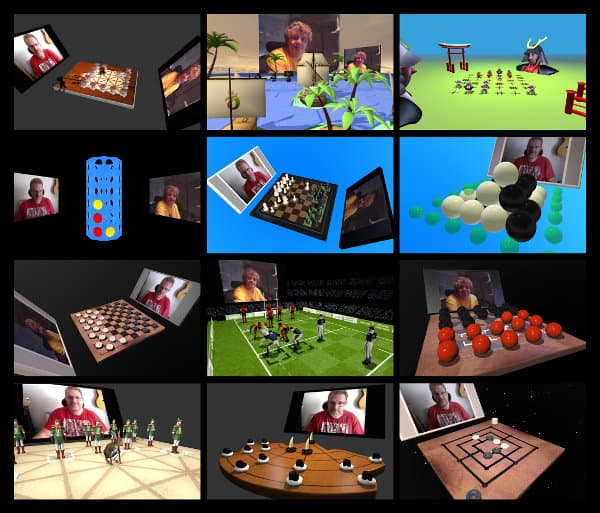
\includegraphics[width=0.75\textwidth]{bilder/jocly-games.jpg}
\caption{Einige Jocly-Spiele, mit WebRTC Telepräsenz.}
\source{\url{https://bloggeek.me/jocly-webrtc-interview/} (Stand 07.05.2021)}
\label{fig:jocly}
\end{figure}

\acs{WebRTC} wird bereits in einigen browserbasierten Mehrspielerspielen, sowie Networking- und Spiel-Frameworks verwendet. In der Regel wird WebRTC jedoch lediglich für Sprach- und Videokommunikation eingesetzt. Die Strategie- und Brettspielplattform \textit{Jocly} ist eine der ersten Plattformen, welche bereits seit 2013 \acs{WebRTC} nutzt, damit Spieler sich in Echtzeit über ihre Webcams beim Spielen sehen, sowie miteinander kommunizieren können (vgl. Abbildung~\ref{fig:jocly}) \cite{jocly2013}.

\begin{figure}[h]
\centering
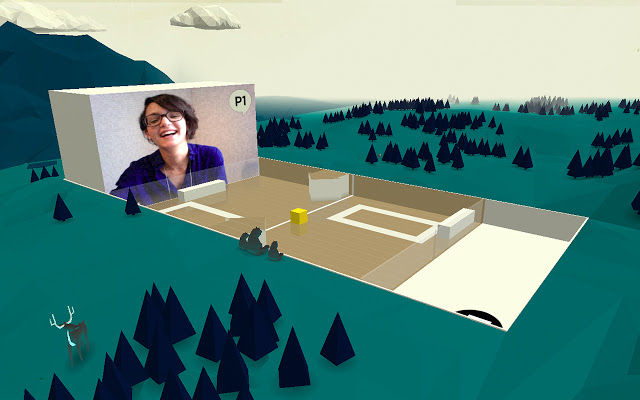
\includegraphics[width=0.75\textwidth]{bilder/cubeslam.jpg}
\caption{Google CubeSlam, mit integriertem WebRTC Videostream.}
\source{\url{https://experiments.withgoogle.com/cube-slam} (Stand 07.05.2021)}
\label{fig:cuubslam}
\end{figure}

Weiterhin existieren eine Reihe an prototypischen Spielen und Frameworks, welche \acs{WebRTC} zum Austausch von Daten nutzen. Bei diesen handelt es sich überwiegend um Echtzeitspiele wie das 2013 von Google entwickelte \textit{CubeSlam}. Abbildung~\ref{fig:cuubslam} zeigt eine Bildschirmaufnahme eines CubeSlam-Spiels. CubeSlam nutzt \acs{WebRTC} Medienstreams um Videodaten zu übertragen, und Datenkanäle, um die Spieldaten zwischen den Spielern zu synchronisieren. Auch der 2012 von Mozilla entwickelte First-Person-Shooter \textit{Bananabread}\footnote{vgl. \url{https://hacks.mozilla.org/2013/03/webrtc-data-channels-for-great-multiplayer/}, Stand 12.05.2021} nutzt WebRTC zum Austausch von Spieldaten.\par

Die Nutzung von WebRTC in (komerziellen) Mehrspielerspielen, Frameworks und Plattformen lässt sich in drei grobe Kategorien aufteilen: Telepräsenz, Datenübertragung, und Render-Streaming. Beispiele für weitere Spiele und Frameworks, welche in diese Kategorien fallen, sind in Tabelle~\ref{table:others} gelistet.

Mehrspielerspiele, welche auf den Videospiel-Engines Godot und Construct2 oder Construct3 basieren, können auch unter Nutzung von WebRTC browserbasiert aufgesetzt werden. Bei diesen Spielen handelt es sich in der Regel aber um Echtzeitspiele, oder diese sind -- im Falle von Brettspielen -- auf maximal zwei Spieler begrenzt\footnote{vgl. \url{https://www.construct.net/en/tutorials/building-basic-board-game-390} und Construct-Mehrspielerspiele: \url{https://www.construct.net/en/free-online-games/multiplayer-7}, Stand: 12.05.2021}.\par 

\addtocounter{footnote}{-2}

\begin{table}[ht]
\centering
\begin{tabularx}{\textwidth}{llX}
\toprule
Software&Nutzung&Beschreibung\\
\midrule
Roll20&Telepräsenz&\glqq{}Roll20\grqq{} ist ein online-Tabletop zum Spielen des Rollenspiels \glqq{}Dungeons and Dragons\grqq{}. Roll20 nutzt WebRTC für Telepräsenz in Form von Audio- und Videochat \cite{roll20}.\\
Tabloro&Telepräsenz&\glqq{}Tabloro\grqq{} ist eine Virtuelle Tabletop-Plattform im Browser. Diese nutzt WebRTC für Telepräsenz in Form von Audio- und Videochat\footnotemark.\\
Construct&Datenübertragung&Die \glqq{}Construct\grqq{} Videospielengine (Construct2 und Construct3) integriert WebRTC zur Datenübertragung zwischen Spielern. Falls WebRTC nicht verwendet werden kann, werden WebSockets verwendet. Spiele, welche auf dieser Engine basieren können auch im Browser gespielt werden \cite{construct}\footnotemark. Die Engine wird primär für 2D-Plattformerspiele verwendet.\\
Godot&Datenübertragung&Die Godot-Engine unterstützt seit 2019 WebRTC zur Datenübertragung \cite{godot}\footnotemark.\\
Unity&Render-Streaming&In der Unity-Engine kann WebRTC verwendet werden, um Bilder, welche auf Hardwarestarken Geräten gerendert wurden, auf Hardwareschwache Geräte zu streamen \cite{unity}.\\
\bottomrule

\end{tabularx}
\caption{Verwendung von WebRTC in Videospiel-Frameworks und Engines.}
\label{table:others}
\end{table}

\newpage

Im Bereich der Rundenbasierten Brettspieleentwicklung im Browser findet WebRTC nur begrenzt Anwendung. Diese beschränkt sich primär auf die zuvor beschriebene Nutzung für Telepräsenz zwischen Spielern.\par

\footnotetext[1]{vgl. \url{https://github.com/fyyyyy/tabloro}, Stand: 12.05.2021}

\footnotetext[2]{vgl. auch \url{https://www.construct.net/en/tutorials/multiplayer-tutorial-concepts-579/connectivity-2}, Stand 12.05.2021}

\footnotetext[3]{vgl. auch \url{https://godotengine.org/article/godot-webrtc-report3}, Stand 12.05.2021}